\documentclass[12pt]{article}
\usepackage[letterpaper,margin=0.62in,headheight=15pt,headsep=15pt,footskip=25pt]{geometry}
\usepackage[T1]{fontenc}
\usepackage{lmodern}
\usepackage{helvet}
\renewcommand{\familydefault}{\sfdefault}
\usepackage{tikz}
\usetikzlibrary{arrows.meta,automata,positioning}
\usepackage{fancyhdr,array,amsmath}
\pagestyle{fancy}
\fancyhf{}
\renewcommand{\headrulewidth}{0.35pt}
\fancyfoot[C]{\fontsize{9}{11}\selectfont Bellingham Math Circle / Week 17 / W17-RV-draft / \thepage}
\setlength{\parindent}{0pt}
\setlength{\parskip}{9pt}
\newcommand{\pageheader}[1]{\fancyhead[C]{\fontsize{11.5}{14}\selectfont Week 17 / Machine memory / #1}}
\newcommand{\problem}[2]{\textbf{Problem #1:} #2\par}
\newcommand{\card}[1]{\tikz[baseline=-0.65ex]{\node[draw,rounded corners=1pt,minimum width=0.28in,minimum height=0.32in,inner sep=2pt,fill=\ifx#1R red!12\else blue!12\fi]{#1};}}
\newcommand{\blankmachine}[1]{\begin{center}\begin{tikzpicture}[x=1in,y=1in]\draw[gray!55,line width=0.5pt] (0,0) rectangle (6.9,#1);\end{tikzpicture}\end{center}}
\newcommand{\rowline}[1]{#1 & \rule[-0.14in]{0pt}{0.50in}\\\hline}
\begin{document}
\fontsize{14}{17.5}\selectfont
\pageheader{Grades K--1 and up}

Read cards from left to right. Start fresh for each new row. Mark one fixed starting state START. Each state has a fixed YES or NO and exactly one fixed R arrow and one fixed B arrow. Follow the arrow for each card, even if it stays put. Hide used cards: the marker's state is the whole memory. Stop anywhere and read YES or NO.

This example machine says YES when the last card is blue.
\begin{center}
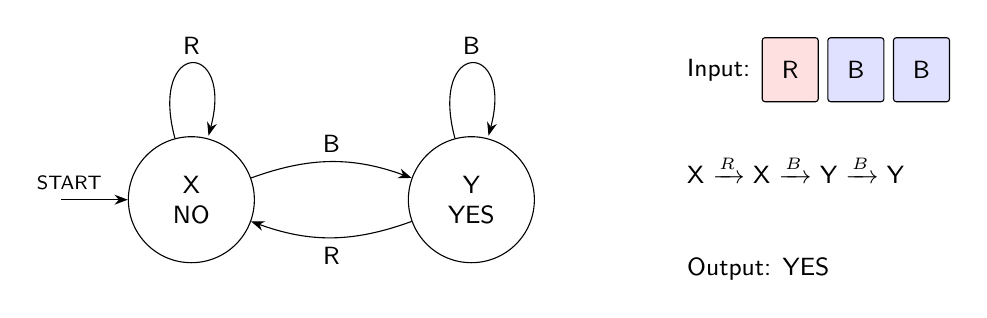
\begin{tikzpicture}[x=1in,y=1in,>=Stealth,font=\small]
  \node[circle,draw,minimum size=0.63in,align=center] (X) at (0.65,0.35) {X\\NO};
  \node[circle,draw,minimum size=0.63in,align=center] (Y) at (2.05,0.35) {Y\\YES};
  \draw[->] (0,0.35)--(X) node[pos=0.12,above,font=\scriptsize] {START};
  \path[->] (X) edge[bend left=20] node[above] {B} (Y)
            (Y) edge[bend left=20] node[below] {R} (X)
            (X) edge[loop above] node {R} (X)
            (Y) edge[loop above] node {B} (Y);
  \node[anchor=west] at (3.08,1.0) {Input: \card{R}\ \card{B}\ \card{B}};
  \node[anchor=west] at (3.08,0.50) {X $\xrightarrow{R}$ X $\xrightarrow{B}$ Y $\xrightarrow{B}$ Y};
  \node[anchor=west] at (3.08,0.0) {Output: YES};
\end{tikzpicture}
\end{center}

\problem{1}{Build a machine that says YES exactly when two red cards in a row have appeared anywhere. It must still say YES after more cards arrive. How few states can it use?}

\begin{center}
\begin{tabular}{@{}c@{\hspace{0.40in}}c@{\hspace{0.40in}}c@{}}
\card{R}\ \card{R}\ \card{B}\ \card{B} &
\card{R}\ \card{B}\ \card{R} &
\card{B}\ \card{R}\ \card{R}\ \card{B}
\end{tabular}
\end{center}
\blankmachine{2.5}
\rule{\linewidth}{0.35pt}
\par\vspace{0.25in}
\rule{\linewidth}{0.35pt}

\newpage
\pageheader{Grades 2--3 and up}
\problem{2}{Build a machine that says YES exactly when the row has an even number of red cards and an even number of blue cards. Zero counts as even. How few states can it use?}

\blankmachine{3.5}
\begin{center}
\renewcommand{\arraystretch}{1.0}
\begin{tabular}{|p{4.8in}|p{1.5in}|}\hline
Row & Machine says\\\hline
\rowline{No cards}
\rowline{\card{R}}
\rowline{\card{R}\ \card{B}}
\rowline{\card{R}\ \card{R}\ \card{B}\ \card{B}}
\rowline{\card{B}\ \card{B}\ \card{R}}
\rowline{\card{B}\ \card{R}\ \card{B}\ \card{R}}
\end{tabular}
\end{center}

\newpage
\pageheader{Grades 4--5}
\problem{3}{Build a machine that says YES exactly when the red and blue counts are equal. Try to defeat a partner's machine with a card row. Could any machine with a fixed number of states work for rows of every length? Explain your answer.}

\begin{center}
\begin{tabular}{@{}c@{\hspace{0.50in}}c@{\hspace{0.50in}}c@{}}
\card{R}\ \card{R}\ \card{B}\ \card{B} &
\card{R}\ \card{B}\ \card{R}\ \card{B} &
\card{B}\ \card{R}\ \card{R}
\end{tabular}
\end{center}
\blankmachine{3.2}
\begin{center}
\renewcommand{\arraystretch}{1.6}
\begin{tabular}{|p{4.4in}|p{1.9in}|}\hline
Row & Machine says\\\hline
\rule{0pt}{0.42in}&\\\hline
\rule{0pt}{0.42in}&\\\hline
\rule{0pt}{0.42in}&\\\hline
\end{tabular}
\end{center}
\vspace{0.16in}
\rule{\linewidth}{0.35pt}
\par\vspace{0.30in}
\rule{\linewidth}{0.35pt}
\par\vspace{0.30in}
\rule{\linewidth}{0.35pt}
\end{document}
